\documentclass[12pt,a4paper,twoside]{article}

% Include packages that contain additional features, for example including special mathematical characters and images in your document
\usepackage{amssymb,amsmath,graphicx}
\usepackage[hidelinks]{hyperref}
\usepackage{verbatim}
%\usepackage{pdfpages}

\title{Exercises IV}
\author{Robin Greif (Exercise 3 Francisco Aros), Lia Hankla (Exercise 2 Victor Ksoll)}
\date{Due 2018/05/11}

\begin{document}
\maketitle

% Lab
\section{Exercise 1: Numerov Algorithm for the Schroedinger Equation}

\begin{figure}[h!]
  \centering
  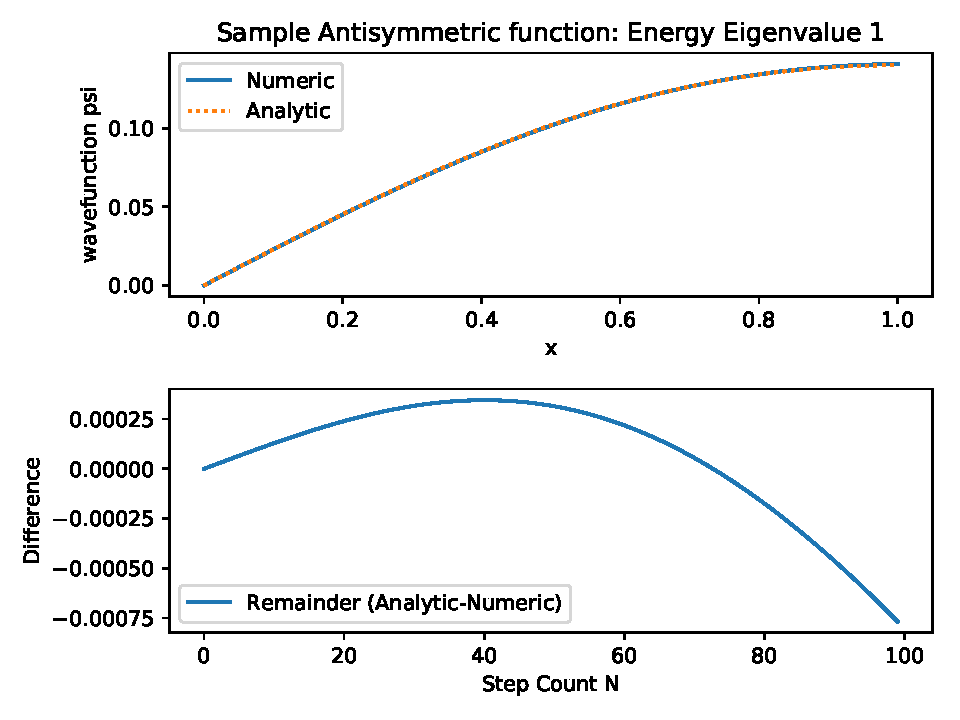
\includegraphics[width=.9\textwidth]{../exercise4_problem1_antisymEx.pdf}
  \caption{Antisymmetric solutions for harmonic oscillator using the Numerov Algorithm, compared to analytic solution} 
  \label{fig:1a}
\end{figure}

\begin{figure}[h!]
  \centering
  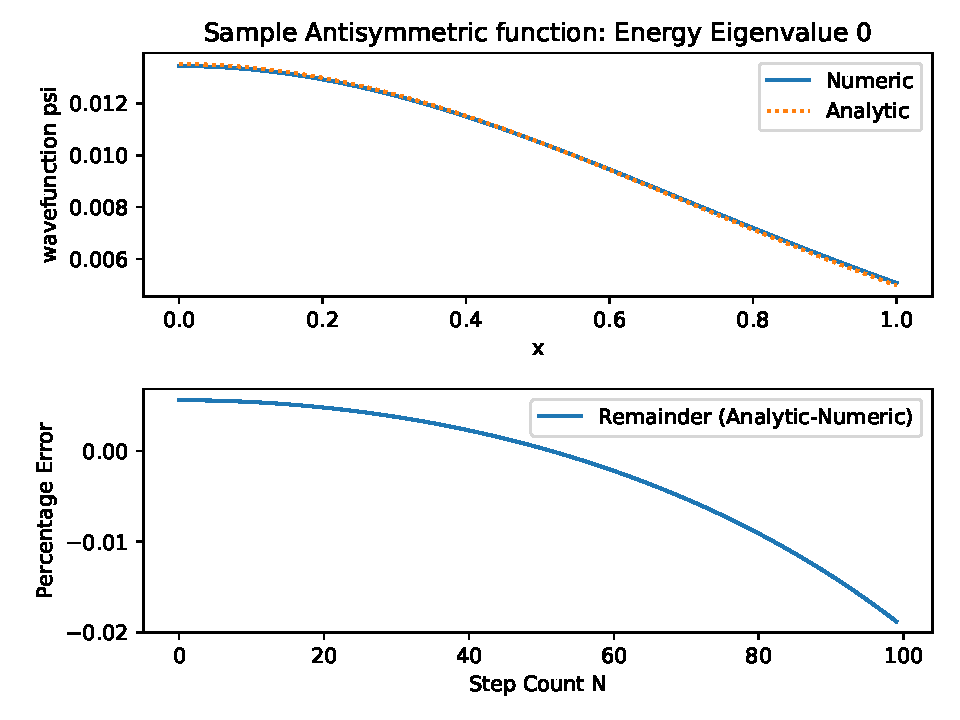
\includegraphics[width=.9\textwidth]{../exercise4_problem1_symEx.pdf}
  \caption{Symmetric solutions for harmonic oscillator using the Numerov Algorithm, compared to analytic solution} 
  \label{fig:1b}
\end{figure}


% Homework
\section*{Exercise 2: Neutrons in the gravitational field}

\begin{align}
  0 &= \bigg(\frac{\hbar^2}{2m} \frac{\partial^2}{\partial z^2} - V(z) \bigg)
            \psi(z) + E \psi(z)  \\     
  0 &= \bigg(\frac{\hbar^2}{2m} \frac{\partial^2}{\partial z^2} - mgz \bigg)
            \psi(z) + E \psi(z)  \\     
  0 &= \bigg(\frac{\hbar^2}{2m} \frac{1}{R^2} \frac{\partial^2}{\partial z^2} - mgRx \bigg)
            \psi(x) + mgR\epsilon \psi(x)  \\       
  0 &= \psi''(x) + (\epsilon - x) \psi(x)  
  \label{eq:neutron_grav}
\end{align}

where we used
\begin{align}
  R &= \bigg( \frac{\hbar^2}{2m^2g} \bigg) ^(1/3)  \\
  x &= z/R = V(x) * \bigg( \frac{1}{mgR} \bigg)  \\
  \epsilon &= \frac{E}{mgR}  
\end{align}

with units
\begin{align}
  [R] &= \bigg( \frac{[Energy \times time]^2}{[mass]^2 [length \times time^{-2}]} \bigg)^{1/3}  \\
      &= [Energy^2 \times time^4 \times mass^{-2} \times length^{-1}]  \\
      &= [[mass \times length^2 \times time^{-2}]^2 \times time^4 \times mass^{-2} \times length^{-1}]  \\
      &= [mass^2 \times length^4 \times time^{-4} \times time^4 \times mass^{-2} \times length^{-1}]  \\
      &= [length^3]  \\
  [x] &= [length]/[length^3] = [length^{-2}] \\
  [\epsilon] &= \frac{[Energy]}{[mass][m][length \times time^{-2}][length^3]}  \\
             &= [Energy \times mass^{-1} \times length^{-1} \times time^2 \times length^{-3} ] \\
             &= [mass \times length^2 \times time^{-2} \times mass^{-1} \times length^{-1} \times time^2 \times length^{-3}]  \\
             &= [length^{-2}]
\end{align}



\subsection*{Part 1}

\begin{figure}[h!]
  \centering
  \includegraphics[width=.9\textwidth]{../exercise4_problem2_numIntegration.pdf}
  \caption{Numerically integrating Eq.~\ref{eq:neutron_grav}, plotted well into the 
            classically forbidden range, $x >> \epsilon$}
  \label{fig:2a}
\end{figure}

For large x, these are supposed to approach $\pm \infty$, however, due to some 
problems in the code, this behavior has not been recovered. Hence, we are unable
to plot one of each. 

In Fig.~\ref{fig:2b}, various values of $\epsilon$ are plotted
showing the recovering of sinusoidal behavior without a damping factor, with the
frequency increasing as $\epsilon$ increases. For $\epsilon<0$, we recovered 
an exponential function. This clearly indicates that the potential function applied
has a problem, specifically, we have no mirror interactions or gravitational effect
visible in the solutions. An explicit integration of the fully specific Equation 
should recover the true behavior, but has not been feasible to be completed to a 
reasonable defree within the timeframe, due to missing the forrest for all the trees.

The picture shows clearly a general solution behavior of a second order ordinary
differential equation, with varying frequencies of the resulting sinusoidal and 
varing order of the exponential.

\begin{figure}[h!]
  \centering
  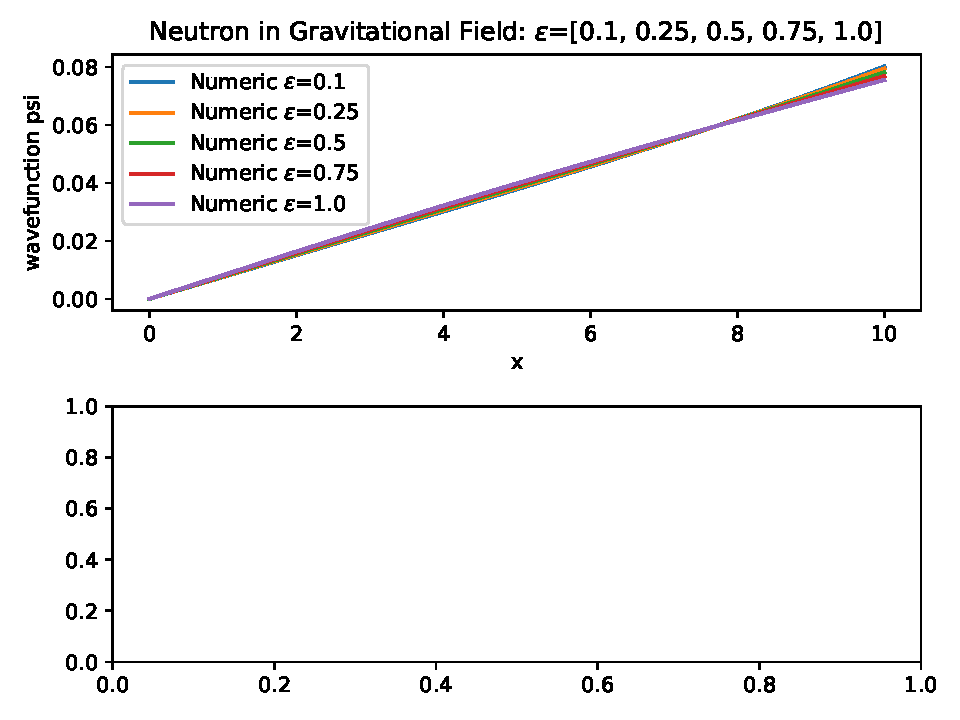
\includegraphics[width=.9\textwidth]{../exercise4_problem2_varyEps.pdf}
  \caption{Numerically integrating Eq.~\ref{eq:neutron_grav} with varying $\epsilon$}
  \label{fig:2b}
\end{figure}



\subsection*{Part 2}

Given that, $\psi(x) \rightarrow 0$ for $x \rightarrow \infty$, 
and increasing $\epsilon_n$ leads to $psi(x)$ changing the sign of its asymptotic
behavior, you can determine the first 3 bound states. The first bound states should correspond
to the first eigentstates where the wavefunction does not diverge. However, due to the lack of a 
proper integration we have been unable to show these, and in fact got an continuously spaced
solution for general non quantized cases. We must sadly concede defeat at this point. However, for those interested the Diplom Thesis of Krantz 2006, has the solutions needed. 
%# eigenvalues, eps_n, belong to normalizable eigenfunctions
%# with psi(x)->0 for x->inf
%# therefore, increasing eps_n => psi(x) changes sign for x->inf
%# a) use this property and eps_n of the first 3 bound states to 2 after comma decimals



%
\subsection*{Appendix: Code}
The code for the exercises is as follows:
\verbatiminput{../exercises04.py}




\end{document}

